\section{Derived Data Description}

The synchronized EEG, fNIRS, EKG and GSR signals generated by the steps described in the previous section are located in the following tables:

\begin{itemize}
	\item eeg\_sync
	\item fnirs\_sync
	\item ekg\_sync
	\item gsr\_sync
\end{itemize}

The column \emph{frequency} indicates the frequency of the shared clock which is 200Hz by default. If we include other frequencies in the feature, the value in this column can be used to select the desired one.

Not all experiments may have data present in the tables due to a couple
of primary reasons. Firstly, time constraints can result in certain tasks
remaining incomplete in some experiments. Secondly, the recorded signals are compromised during certain tasks can also lead to the absence of signals in the tables.

In cases where only two participants participated in the sections, signals for the third participant are spurious but they were synchronized and saved to the sync tables for a computational choice. However, they can be filtered out by joining with the \emph{data\_validity} table. 

\autoref{tab:EEG_signals}, \autoref{tab:fNIRS_raw_signals} and \autoref{tab:fNIRS_signals} detail the mapping between the montage in \autoref{fig:combined-montage} and the naming convention used in the EEG and fNIRS sync tables.

\begin{figure}
  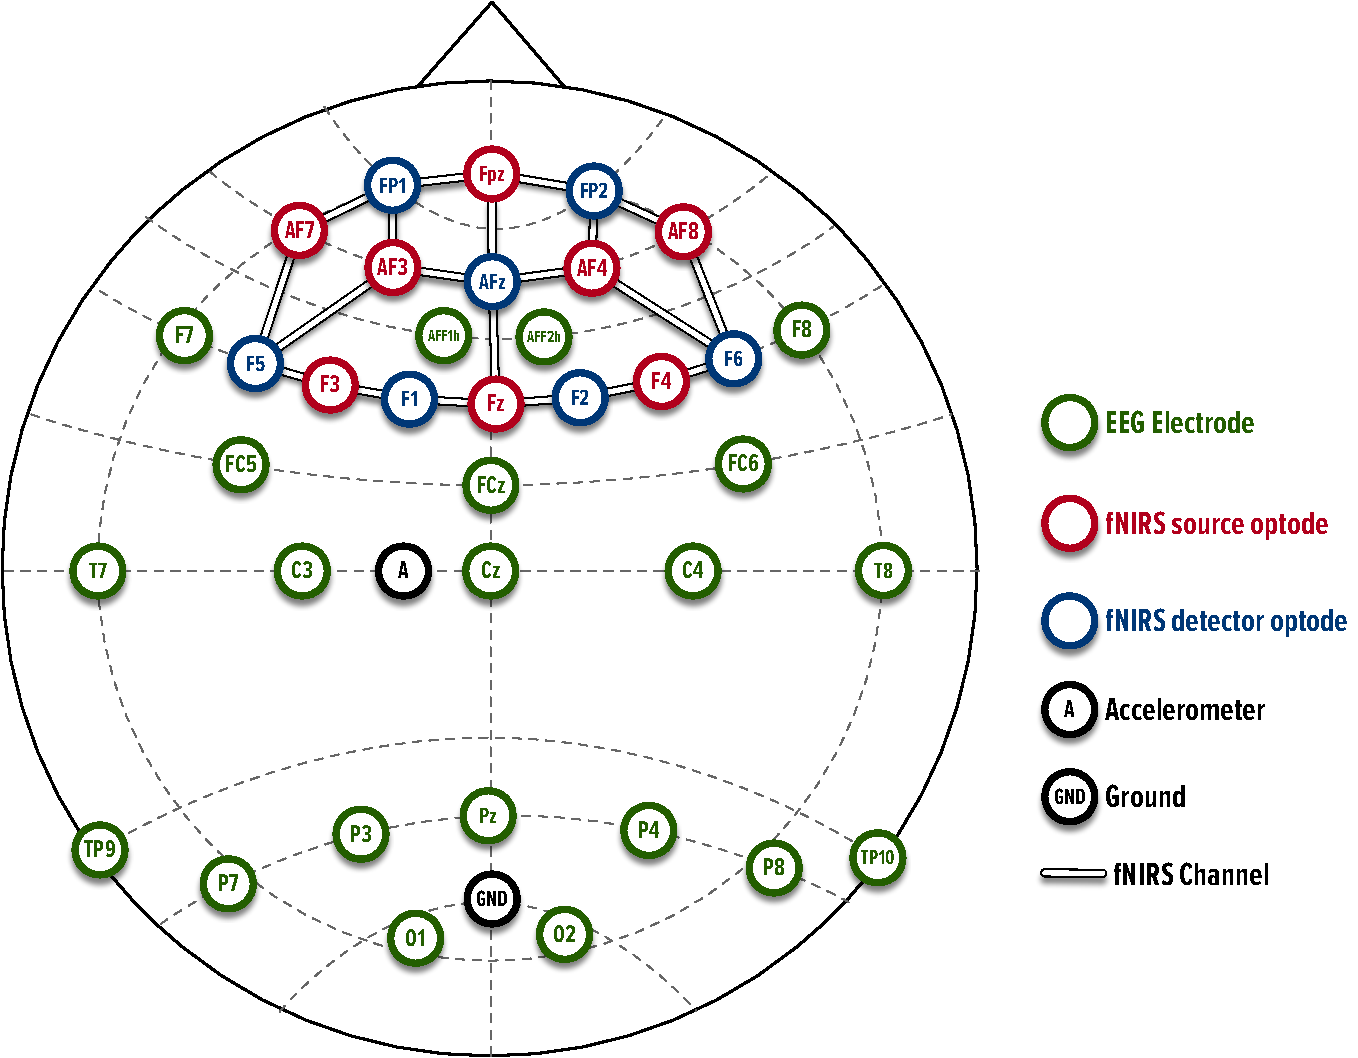
\includegraphics[width=\linewidth]{images/combined_montage.pdf}
  \centering
  \caption{%
      The montage we used for combined EEG/fNIRS data acquisition.  EEG
      electrodes were located in the anterior frontal (AFF1h, AFF2h), frontal
      (F7, F8), frontocentral (FC5, FCz, FC6), central (C3, Cz, C4),
      occipital (O1, O2), temporal (T7, T8) and parietal (P7, P3, Pz, P4, P8)
      regions.  fNIRS optodes were located in frontal (Fz, F1, F2, F3, F4,
      F5, F6), anterior frontal (AF3, AF4, AFz, AF7, AF8), frontal polar
      (FP1, FPz, FP2). The line is the channel formed when fNIRS source
      optode (red) and fNIRS detector (blue) optode are combined.
  }
  \label{fig:combined-montage}
\end{figure}

\begin{table}
\centering
\begin{tabularx}{\textwidth}{lX}
    \toprule
    EEG signal columns & Description (topological location of the subject's brain) \\
    \midrule
    \texttt{<subject>\_eeg\_AFF1h} & Left anterior frontal region \\
    \texttt{<subject>\_eeg\_F7} & Left frontal region  \\
    \texttt{<subject>\_eeg\_FC5} & Left fronto-central region  \\
    \texttt{<subject>\_eeg\_C3} & Left central region \\
    \texttt{<subject>\_eeg\_T7} & Left temporal region \\
    \texttt{<subject>\_eeg\_TP9} & Left temporal-parietal region \\
    \texttt{<subject>\_eeg\_Pz} & Central parietal region \\
    \texttt{<subject>\_eeg\_P3} & Left parietal region \\
    \texttt{<subject>\_eeg\_P7} & Left parietal region \\
    \texttt{<subject>\_eeg\_O1} & Left occipital region \\
    \texttt{<subject>\_eeg\_O2} & Right occipital region \\
    \texttt{<subject>\_eeg\_P8} & Right parietal region \\
    \texttt{<subject>\_eeg\_P4} & Right parietal region \\
    \texttt{<subject>\_eeg\_TP10} & Right temporal-parietal region \\
    \texttt{<subject>\_eeg\_Cz} & central region \\
    \texttt{<subject>\_eeg\_C4} & Right central region \\
    \texttt{<subject>\_eeg\_T8} & Right temporal region \\
    \texttt{<subject>\_eeg\_FC6} & Right fronto-central region \\
    \texttt{<subject>\_eeg\_FCz} & Central fronto-central region \\
    \texttt{<subject>\_eeg\_F8} & Right frontal region \\
    \texttt{<subject>\_eeg\_AFF2h} & Right anterior frontal region \\
    \bottomrule
\end{tabularx}
\caption{EEG signal descriptions, specifying the topological locations on the subject's brain. Each entry provides the label of the signal column corresponding to the EEG electrode location. For a visual representation of these electrode locations, refer to \autoref{fig:combined-montage}.
}
\label{tab:EEG_signals}
\end{table}

\begin{table}
  \footnotesize
  \centering
  \begin{tabularx}{\textwidth}{lX}
  \toprule
  fNIRS raw signal columns & Description (topological location of the subject's brain) \\
  \midrule
  \texttt{<subject>\_fnirs\_S1-D1\_760} & 'F3-F5': left frontal region \\
  \texttt{<subject>\_fnirs\_S1-D2\_760} & 'F3-F1': left frontal region  \\
  \texttt{<subject>\_fnirs\_S2-D1\_760} & 'Af7-F5': left anterior frontal region  \\
  \texttt{<subject>\_fnirs\_S2-D3\_760} & 'Af7-Fp1': left anterior frontal region  \\
  \texttt{<subject>\_fnirs\_S3-D1\_760} & 'Af3-F5': left anterior frontal region  \\
  \texttt{<subject>\_fnirs\_S3-D3\_760} & 'Af3-Fp1': left anterior frontal region  \\
  \texttt{<subject>\_fnirs\_S3-D4\_760} & 'Af3-Afz': left anterior frontal region  \\
  \texttt{<subject>\_fnirs\_S4-D2\_760} & 'Fz-F1': left frontal region  \\
  \texttt{<subject>\_fnirs\_S4-D4\_760} & 'Fz-Afz': central frontal region  \\
  \texttt{<subject>\_fnirs\_S4-D5\_760} & 'Fz-F2': right frontal region  \\
  \texttt{<subject>\_fnirs\_S5-D3\_760} & 'Fpz-Fp1': left frontal polar region  \\
  \texttt{<subject>\_fnirs\_S5-D4\_760} & 'Fpz-Afz': central frontal polar region  \\
  \texttt{<subject>\_fnirs\_S5-D6\_760} & 'Fpz-Fp2': right frontal polar region  \\
  \texttt{<subject>\_fnirs\_S6-D4\_760} & 'Af4-Afz': right anterior frontal region  \\
  \texttt{<subject>\_fnirs\_S6-D6\_760} & 'Af4-Fp2': right anterior frontal region  \\
  \texttt{<subject>\_fnirs\_S6-D7\_760} & 'Af4-F6': right anterior frontal region  \\
  \texttt{<subject>\_fnirs\_S7-D5\_760} & 'F4-F2': right frontal region  \\
  \texttt{<subject>\_fnirs\_S7-D7\_760} & 'F4-F6': right frontal region  \\
  \texttt{<subject>\_fnirs\_S8-D6\_760} & 'Af8-Fp2': right anterior frontal region  \\
  \texttt{<subject>\_fnirs\_S8-D7\_760} & 'Af8-F6': right anterior frontal region  \\
  \texttt{<subject>\_fnirs\_S1-D1\_850} & 'F3-F5': left frontal region  \\
  \texttt{<subject>\_fnirs\_S1-D2\_850} & 'F3-F1': left frontal region  \\
  \texttt{<subject>\_fnirs\_S2-D1\_850} & 'Af7-F5': left anterior frontal region  \\
  \texttt{<subject>\_fnirs\_S2-D3\_850} & 'Af7-Fp1': left anterior frontal region  \\
  \texttt{<subject>\_fnirs\_S3-D1\_850} & 'Af3-F5': left anterior frontal region  \\
  \texttt{<subject>\_fnirs\_S3-D3\_850} & 'Af3-Fp1': left anterior frontal region  \\
  \texttt{<subject>\_fnirs\_S3-D4\_850} & 'Af3-Afz': left anterior frontal region  \\
  \texttt{<subject>\_fnirs\_S4-D2\_850} & 'Fz-F1': left frontal region  \\
  \texttt{<subject>\_fnirs\_S4-D4\_850} & 'Fz-Afz': central frontal region  \\
  \texttt{<subject>\_fnirs\_S4-D5\_850} & 'Fz-F2': right frontal region  \\
  \texttt{<subject>\_fnirs\_S5-D3\_850} & 'Fpz-Fp1': left frontal polar region  \\
  \texttt{<subject>\_fnirs\_S5-D4\_850} & 'Fpz-Afz': central frontal polar region  \\
  \texttt{<subject>\_fnirs\_S5-D6\_850} & 'Fpz-Fp2': right frontal polar region  \\
  \texttt{<subject>\_fnirs\_S6-D4\_850} & 'Af4-Afz': right anterior frontal region  \\
  \texttt{<subject>\_fnirs\_S6-D6\_850} & 'Af4-Fp2': right anterior frontal region  \\
  \texttt{<subject>\_fnirs\_S6-D7\_850} & 'Af4-F6': right anterior frontal region  \\
  \texttt{<subject>\_fnirs\_S7-D5\_850} & 'F4-F2': right frontal region  \\
  \texttt{<subject>\_fnirs\_S7-D7\_850} & 'F4-F6': right frontal region  \\
  \texttt{<subject>\_fnirs\_S8-D6\_850} & 'Af8-Fp2': right anterior frontal region  \\
  \texttt{<subject>\_fnirs\_S8-D7\_850} & 'Af8-F6': right anterior frontal region  \\
  \bottomrule
  \end{tabularx}
  \caption{Table of fNIRS raw signal descriptions, mapping the source (S) to the detector (D) for various topological locations on the subject's brain. These signals where recorded using the Aurora fNIRS software. Each channel is recorded using light wavelengths of 760nm and 850nm. For a visual representation of these electrode locations, refer to \autoref{fig:combined-montage}.}
  \label{tab:fNIRS_raw_signals}
  \end{table}

  \begin{table}
      \footnotesize
    \centering
    \begin{tabularx}{\textwidth}{lX}
    \toprule
    fNIRS raw signal columns & Description (topological location of the subject's brain) \\
    \midrule
    \texttt{<subject>\_fnirs\_S1-D1\_HbO} & 'F3-F5': left frontal region \\
    \texttt{<subject>\_fnirs\_S1-D2\_HbO} & 'F3-F1': left frontal region  \\
    \texttt{<subject>\_fnirs\_S2-D1\_HbO} & 'Af7-F5': left anterior frontal region  \\
    \texttt{<subject>\_fnirs\_S2-D3\_HbO} & 'Af7-Fp1': left anterior frontal region  \\
    \texttt{<subject>\_fnirs\_S3-D1\_HbO} & 'Af3-F5': left anterior frontal region  \\
    \texttt{<subject>\_fnirs\_S3-D3\_HbO} & 'Af3-Fp1': left anterior frontal region  \\
    \texttt{<subject>\_fnirs\_S3-D4\_HbO} & 'Af3-Afz': left anterior frontal region  \\
    \texttt{<subject>\_fnirs\_S4-D2\_HbO} & 'Fz-F1': left frontal region  \\
    \texttt{<subject>\_fnirs\_S4-D4\_HbO} & 'Fz-Afz': central frontal region  \\
    \texttt{<subject>\_fnirs\_S4-D5\_HbO} & 'Fz-F2': right frontal region  \\
    \texttt{<subject>\_fnirs\_S5-D3\_HbO} & 'Fpz-Fp1': left frontal polar region  \\
    \texttt{<subject>\_fnirs\_S5-D4\_HbO} & 'Fpz-Afz': central frontal polar region  \\
    \texttt{<subject>\_fnirs\_S5-D6\_HbO} & 'Fpz-Fp2': right frontal polar region  \\
    \texttt{<subject>\_fnirs\_S6-D4\_HbO} & 'Af4-Afz': right anterior frontal region  \\
    \texttt{<subject>\_fnirs\_S6-D6\_HbO} & 'Af4-Fp2': right anterior frontal region  \\
    \texttt{<subject>\_fnirs\_S6-D7\_HbO} & 'Af4-F6': right anterior frontal region  \\
    \texttt{<subject>\_fnirs\_S7-D5\_HbO} & 'F4-F2': right frontal region  \\
    \texttt{<subject>\_fnirs\_S7-D7\_HbO} & 'F4-F6': right frontal region  \\
    \texttt{<subject>\_fnirs\_S8-D6\_HbO} & 'Af8-Fp2': right anterior frontal region  \\
    \texttt{<subject>\_fnirs\_S8-D7\_HbO} & 'Af8-F6': right anterior frontal region  \\
    \texttt{<subject>\_fnirs\_S1-D1\_HbR} & 'F3-F5': left frontal region  \\
    \texttt{<subject>\_fnirs\_S1-D2\_HbR} & 'F3-F1': left frontal region  \\
    \texttt{<subject>\_fnirs\_S2-D1\_HbR} & 'Af7-F5': left anterior frontal region  \\
    \texttt{<subject>\_fnirs\_S2-D3\_HbR} & 'Af7-Fp1': left anterior frontal region  \\
    \texttt{<subject>\_fnirs\_S3-D1\_HbR} & 'Af3-F5': left anterior frontal region  \\
    \texttt{<subject>\_fnirs\_S3-D3\_HbR} & 'Af3-Fp1': left anterior frontal region  \\
    \texttt{<subject>\_fnirs\_S3-D4\_HbR} & 'Af3-Afz': left anterior frontal region  \\
    \texttt{<subject>\_fnirs\_S4-D2\_HbR} & 'Fz-F1': left frontal region  \\
    \texttt{<subject>\_fnirs\_S4-D4\_HbR} & 'Fz-Afz': central frontal region  \\
    \texttt{<subject>\_fnirs\_S4-D5\_HbR} & 'Fz-F2': right frontal region  \\
    \texttt{<subject>\_fnirs\_S5-D3\_HbR} & 'Fpz-Fp1': left frontal polar region  \\
    \texttt{<subject>\_fnirs\_S5-D4\_HbR} & 'Fpz-Afz': central frontal polar region  \\
    \texttt{<subject>\_fnirs\_S5-D6\_HbR} & 'Fpz-Fp2': right frontal polar region  \\
    \texttt{<subject>\_fnirs\_S6-D4\_HbR} & 'Af4-Afz': right anterior frontal region  \\
    \texttt{<subject>\_fnirs\_S6-D6\_HbR} & 'Af4-Fp2': right anterior frontal region  \\
    \texttt{<subject>\_fnirs\_S6-D7\_HbR} & 'Af4-F6': right anterior frontal region  \\
    \texttt{<subject>\_fnirs\_S7-D5\_HbR} & 'F4-F2': right frontal region  \\
    \texttt{<subject>\_fnirs\_S7-D7\_HbR} & 'F4-F6': right frontal region  \\
    \texttt{<subject>\_fnirs\_S8-D6\_HbR} & 'Af8-Fp2': right anterior frontal region  \\
    \texttt{<subject>\_fnirs\_S8-D7\_HbR} & 'Af8-F6': right anterior frontal region  \\
    \bottomrule
    \end{tabularx}
    \caption{%
        fNIRS raw signal descriptions, mapping the source (S) to the detector
        (D) for various topological locations on the subject's brain. HbO, or
        oxyhemoglobin, and HbR, or deoxyhemoglobin, are the two types of
        hemoglobin measured. For a visual representation of these electrode
        locations, refer to \autoref{fig:combined-montage}.
    }
    \label{tab:fNIRS_signals}
    \end{table}
